\documentclass[10pt]{article}
\usepackage[utf8]{inputenc}
\usepackage[T1]{fontenc}
\usepackage{amsmath}
\usepackage{amsfonts}
\usepackage{amssymb}
\usepackage[version=4]{mhchem}
\usepackage{stmaryrd}
\usepackage{bbold}
\usepackage{graphicx}
\usepackage[export]{adjustbox}
\graphicspath{ {./images/} }

\begin{document}
\subsection{This is achieveable!}
Perhaps remarkably, this last goal is actually achieveable, in a very general way. As we will see in the coming sections, we can start with any algorithm that produces a "point predictor" $\hat{f}_{n}$ that predicts $Y_{n+1}$ from $X_{n+1}$, and turn this into a "set predictor" $\hat{C}_{n}$ that satisfies (1).

The basic idea behind conformal prediction is two-fold. The first key idea can actually be explained in a simpler context, where there are no features at all, and we just have a sequence $Y_{i} \in \mathbb{R}, i=1, \ldots, n$ of real-valued response values. Suppose our goal is to find a one-sided prediction interval $\hat{C}_{n}=\left(-\infty, \hat{q}_{n}\right]$ with

\begin{center}
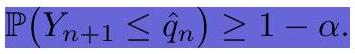
\includegraphics[max width=\textwidth]{2023_10_05_3f4b7f0ae8e12ec8ac84g-02}
\end{center}

Given this goal (2), a natural place to start would be to set $\hat{q}_{n}$ to be the level $(1-\alpha)$ sample quantile of $Y_{1}, \ldots, Y_{n}$, which we denote by

\begin{center}
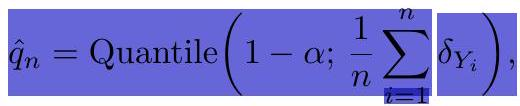
\includegraphics[max width=\textwidth]{2023_10_05_3f4b7f0ae8e12ec8ac84g-02(1)}
\end{center}

with $\delta_{a}$ denoting a point mass at $a$, and hence $\frac{1}{n} \sum_{i=1}^{n} \delta_{Y_{i}}$ denoting the empirical distribution of $Y_{1}, \ldots, Y_{n}$. But this would only give use the approximate result

$\mathbb{P}\left(Y_{n+1} \leq \hat{q}_{n}\right) \approx 1-\alpha$.

This becomes exact as $n \rightarrow \infty$, under standard conditions (that ensure convergence of the sample quantile to the population quantile). So can we instead get something that satisfies (2) in finite-sample?

First key idea: use ranks to form adjusted quantiles. This is where the first key idea behind conformal prediction comes in (which in a sense traces back to work on rank-based statistics and permutations by Fisher and Pitman in the 1930s). As $Y_{n+1}$ is i.i.d. with $Y_{1}, \ldots, Y_{n}$, then

the rank of $Y_{n+1}$ is uniformly distributed over the values $Y_{1}, \ldots, Y_{n+1}$.

This means that

$$
\mathbb{P}\left(Y_{n+1} \text { is among the }\lceil(1-\alpha)(n+1)\rceil \text { smallest of } Y_{1}, \ldots, Y_{n+1}\right) \geq 1-\alpha,
$$

which is in turn equivalent to ${ }^{1}$

$$
\mathbb{P}\left(Y_{n+1} \text { is among the }\lceil(1-\alpha)(n+1)\rceil \text { smallest of } Y_{1}, \ldots, Y_{n}\right) \geq 1-\alpha .
$$

The last step is critical: note that we have moved from a comparison between $Y_{n+1}$ and a an order statistic of $Y_{1}, \ldots, Y_{n+1}$ in (4) to a comparison between $Y_{n+1}$ and an order statistic of $Y_{1}, \ldots, Y_{n}$ in (5). This is key, because what is on the right-hand side of the $\leq$ sign in (5) is computable from just the first $n$ points. Accordingly, by defining

$$
\hat{q}_{n}=\lceil(1-\alpha)(n+1)\rceil \text { smallest of } Y_{1}, \ldots, Y_{n},
$$

\section{we have precisely achieved (2).}
The formulation in (6) is arguably the most intuitive way to remember how to achieve coverage. There are other equivalent formulations. One such equivalent formulation (we will see more later on) is

\begin{center}
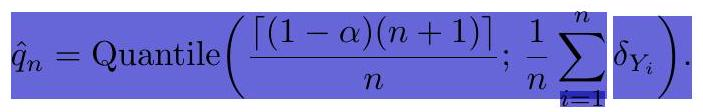
\includegraphics[max width=\textwidth]{2023_10_05_3f4b7f0ae8e12ec8ac84g-02(2)}
\end{center}

${ }^{1}$ To see this, consider the complement of the events (inside the probabilities) in (4), (5). Abbreviate $k=\lceil(1-\alpha)(n+1)]$. Then $Y_{n+1}>$ the $k$ smallest of $Y_{1}, \ldots, Y_{n+1}$ is clearly an equivalent statement to $Y_{n+1}>$ the $k$ smallest of $Y_{1}, \ldots, Y_{n}$, since $Y_{n+1}$ can never be strictly larger than itself. That said, this argument really only makes sense for $k \leq n$, and for $k=n+1$, which occurs if $\alpha<1 /(n+1)$, then $[(1-\alpha)(n+1)]=n+1$, then we have to interpret the $(n+1)$ smallest of $Y_{1}, \ldots, Y_{n}$ as being $+\infty$ to equate (4), (5). This is the consistent with interpreting the quantile function in (7) to return $+\infty$ when the input level is $\geq 1$. In this way, we can also see the solution here as simply to taking the sample quantile at an adjusted level: we use $\lceil(1-\alpha)(n+1)\rceil / n$, instead of $1-\alpha$, which is a sort of finite-sample correction. But in our opinion, the fact that (7) achieves the coverage guarantee is less obvious; only through its equivalence to (6) - and then the equivalence to the precedings displays in (5), (4), (3)-does this become transparent. A very simple illustration of the key idea here is given in Figure 1.

\begin{center}
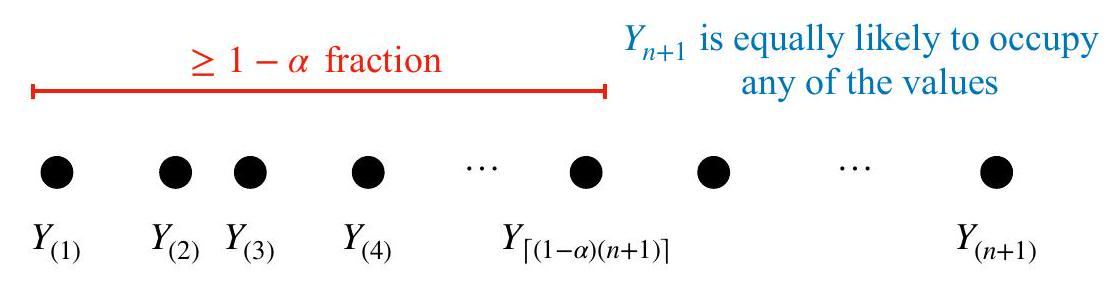
\includegraphics[max width=\textwidth]{2023_10_05_3f4b7f0ae8e12ec8ac84g-03}
\end{center}

Figure 1: Illustration of the first key idea in conformal prediction, as stated in (3), (4). Note also that we have the sharpened version (8) when there are almost surely no ties.

Love Exchangeability is all you need. Looking back at (3), all that we need for this to hold is that $Y_{1}, \ldots, Y_{n+1}$ are exchangeable, which is a weaker than the i.i.d. assumption. Recall that exchangeability of $Y_{1}, \ldots, Y_{n+1}$ means that their joint distribution is unchanged under permutations:

$$
\left(Y_{1}, \ldots, Y_{n+1}\right) \stackrel{d}{=}\left(Y_{\sigma(1)}, \ldots, Y_{\sigma(n+1)}\right), \text { for all permutations } \sigma
$$

Coverage upper bound when there are no ties. If there are almost surely no ties between $Y_{1}, \ldots, Y_{n+1}$ (or we use a suitably random tie-breaking rule) then the statement in (4) can be sharpened to an equality,

$$
\mathbb{P}\left(Y_{n+1} \text { is among the }\lceil(1-\alpha)(n+1)\rceil \text { smallest of } Y_{1}, \ldots, Y_{n+1}\right)=\frac{\lceil(1-\alpha)(n+1)\rceil}{n+1} .
$$

Simply upper bounding the right-hand side above gives

$$
\mathbb{P}\left(Y_{n+1} \text { is among the }\lceil(1-\alpha)(n+1)\rceil \text { smallest of } Y_{1}, \ldots, Y_{n+1}\right)<(1-\alpha)+\frac{1}{n+1} .
$$

Carrying on from by the same logic as before leads to the sharpened conclusion,

$$
\mathbb{P}\left(Y_{n+1} \leq \hat{q}_{n}\right) \in\left[1-\alpha, 1-\alpha+\frac{1}{n+1}\right)
$$

with $\hat{q}_{n}$ still defined as in (6). To be clear, the lower bound on coverage in (10) always holds, and the upper bound holds under the assumption that there are almost surely no ties.

Naive attempt to lift this idea to regression problems. Now let's try to lift the first key idea to a regression setting, where we observe both $X_{i} \in \mathcal{X}$ and $Y_{i} \in \mathbb{R}, i=1, \ldots, n$, and want a prediction set for $Y_{n+1}$ based on $X_{n+1}$. Suppose that $\hat{f}_{n}$ is any point predictor, trained on $\left(X_{i}, Y_{i}\right), i=1, \ldots, n$, such that (to put it informally)

$$
\hat{f}_{n}(x) \text { predicts the value of } y \text { that we expect to see at } x \text {. }
$$

Then we could proceed naively as follows. We define (absolute) residuals made on the training set,

$$
R_{i}=\left|Y_{i}-\hat{f}_{n}\left(X_{i}\right)\right|, \quad i=1, \ldots, n,
$$

and just as in (6), let $\hat{q}_{n}=\lceil(1-\alpha)(n+1)\rceil$ smallest of $R_{1}, \ldots, R_{n}$. We could then define the prediction set to be $\hat{C}_{n}(x)=\left\{y:\left|y-\hat{f}_{n}(x)\right| \leq \hat{q}_{n}\right\}$, or in other words

$$
\hat{C}_{n}(x)=\left[\hat{f}_{n}(x)-\hat{q}_{n}, \hat{f}_{n}(x)+\hat{q}_{n}\right]
$$


\end{document}